% Auto-generated by scripts/export_excited_mass_table.py
\begin{figure}[ht]
\centering
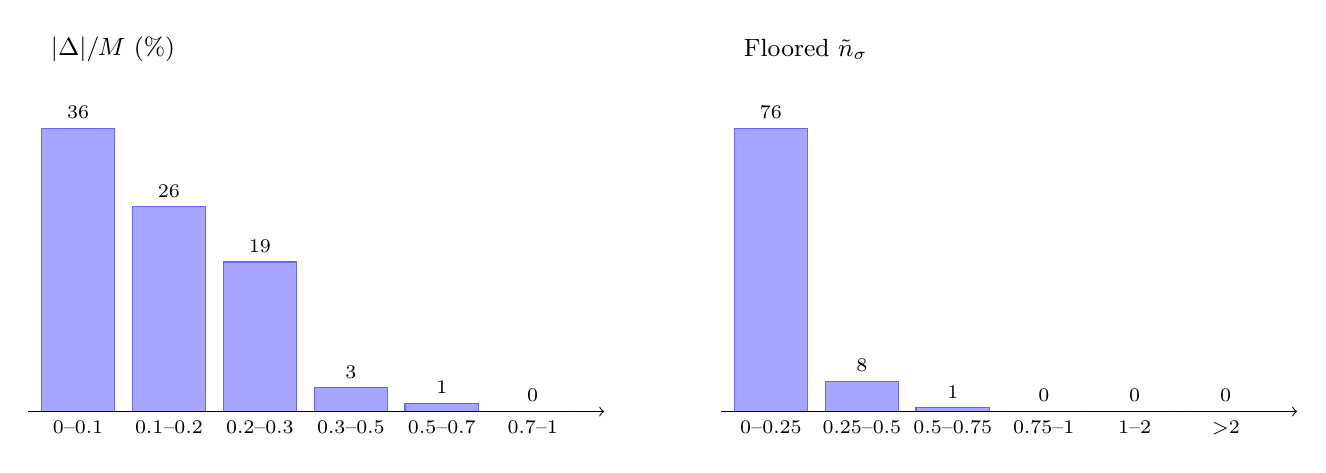
\begin{tikzpicture}[x=1.1cm,y=1cm]
\node[anchor=west] at (0.0, 4.6) {\small $|\Delta|/M$ (\%)};
\draw[fill=blue!35,draw=blue!60] (0.0,0) rectangle (0.85,3.600);
\node[anchor=north,font=\scriptsize] at (0.425,0) {0--0.1};
\node[anchor=south,font=\scriptsize] at (0.425,3.600) {36};
\draw[fill=blue!35,draw=blue!60] (1.05,0) rectangle (1.9,2.600);
\node[anchor=north,font=\scriptsize] at (1.475,0) {0.1--0.2};
\node[anchor=south,font=\scriptsize] at (1.475,2.600) {26};
\draw[fill=blue!35,draw=blue!60] (2.1,0) rectangle (2.95,1.900);
\node[anchor=north,font=\scriptsize] at (2.525,0) {0.2--0.3};
\node[anchor=south,font=\scriptsize] at (2.525,1.900) {19};
\draw[fill=blue!35,draw=blue!60] (3.1500000000000004,0) rectangle (4.0,0.300);
\node[anchor=north,font=\scriptsize] at (3.575,0) {0.3--0.5};
\node[anchor=south,font=\scriptsize] at (3.575,0.300) {3};
\draw[fill=blue!35,draw=blue!60] (4.2,0) rectangle (5.05,0.100);
\node[anchor=north,font=\scriptsize] at (4.625,0) {0.5--0.7};
\node[anchor=south,font=\scriptsize] at (4.625,0.100) {1};
\draw[fill=blue!35,draw=blue!60] (5.25,0) rectangle (6.1,0.000);
\node[anchor=north,font=\scriptsize] at (5.675,0) {0.7--1};
\node[anchor=south,font=\scriptsize] at (5.675,0.000) {0};
\draw[->] (-0.15,0) -- (6.500000000000001,0);
\node[anchor=west] at (8.0, 4.6) {\small Floored $\tilde n_\sigma$};
\draw[fill=blue!35,draw=blue!60] (8.0,0) rectangle (8.85,3.600);
\node[anchor=north,font=\scriptsize] at (8.425,0) {0--0.25};
\node[anchor=south,font=\scriptsize] at (8.425,3.600) {76};
\draw[fill=blue!35,draw=blue!60] (9.05,0) rectangle (9.9,0.379);
\node[anchor=north,font=\scriptsize] at (9.475000000000001,0) {0.25--0.5};
\node[anchor=south,font=\scriptsize] at (9.475000000000001,0.379) {8};
\draw[fill=blue!35,draw=blue!60] (10.1,0) rectangle (10.95,0.047);
\node[anchor=north,font=\scriptsize] at (10.525,0) {0.5--0.75};
\node[anchor=south,font=\scriptsize] at (10.525,0.047) {1};
\draw[fill=blue!35,draw=blue!60] (11.15,0) rectangle (12.0,0.000);
\node[anchor=north,font=\scriptsize] at (11.575000000000001,0) {0.75--1};
\node[anchor=south,font=\scriptsize] at (11.575000000000001,0.000) {0};
\draw[fill=blue!35,draw=blue!60] (12.2,0) rectangle (13.049999999999999,0.000);
\node[anchor=north,font=\scriptsize] at (12.625,0) {1--2};
\node[anchor=south,font=\scriptsize] at (12.625,0.000) {0};
\draw[fill=blue!35,draw=blue!60] (13.25,0) rectangle (14.1,0.000);
\node[anchor=north,font=\scriptsize] at (13.675,0) {$>$2};
\node[anchor=south,font=\scriptsize] at (13.675,0.000) {0};
\draw[->] (7.85,0) -- (14.5,0);
\end{tikzpicture}
\caption{Excited-state mass panel ($85$ PDG rows): histogram of scale-free errors $|\Delta|/M$ (left) and diagnostic floored pulls $\tilde n_\sigma=|\Delta|/\max(\sigma,0.01M)$ (right). Type~A listed-$\sigma$ pulls are audit-only (Table~\ref{tab:listed-pull-extremes}). Listed $\sigma$ source: PDG 2024 RPP (Workman et al., Phys. Rev. D 110, 030001, 2024). Per-state values in \texttt{data/excited\_mass\_panel\_audit.csv}.}
\label{fig:excited-mass-pull-histogram}
\end{figure}
